\PassOptionsToPackage{unicode=true}{hyperref} % options for packages loaded elsewhere
\PassOptionsToPackage{hyphens}{url}
%
\documentclass[
  12pt,
  lettersizepaper,
]{book}
\usepackage{lmodern}
\usepackage{amssymb,amsmath}
\usepackage{ifxetex,ifluatex}
\ifnum 0\ifxetex 1\fi\ifluatex 1\fi=0 % if pdftex
  \usepackage[T1]{fontenc}
  \usepackage[utf8]{inputenc}
  \usepackage{textcomp} % provides euro and other symbols
\else % if luatex or xelatex
  \usepackage{unicode-math}
  \defaultfontfeatures{Scale=MatchLowercase}
  \defaultfontfeatures[\rmfamily]{Ligatures=TeX,Scale=1}
\fi
% use upquote if available, for straight quotes in verbatim environments
\IfFileExists{upquote.sty}{\usepackage{upquote}}{}
\IfFileExists{microtype.sty}{% use microtype if available
  \usepackage[]{microtype}
  \UseMicrotypeSet[protrusion]{basicmath} % disable protrusion for tt fonts
}{}
\makeatletter
\@ifundefined{KOMAClassName}{% if non-KOMA class
  \IfFileExists{parskip.sty}{%
    \usepackage{parskip}
  }{% else
    \setlength{\parindent}{0pt}
    \setlength{\parskip}{6pt plus 2pt minus 1pt}}
}{% if KOMA class
  \KOMAoptions{parskip=half}}
\makeatother
\usepackage{xcolor}
\IfFileExists{xurl.sty}{\usepackage{xurl}}{} % add URL line breaks if available
\IfFileExists{bookmark.sty}{\usepackage{bookmark}}{\usepackage{hyperref}}
\hypersetup{
  pdftitle={This is the title},
  pdfauthor={My Full Name},
  pdfborder={0 0 0},
  breaklinks=true}
\urlstyle{same}  % don't use monospace font for urls
\usepackage[margin=1in, bottom=1in, top=1in, footskip=0.25in, headheight=0.5in]{geometry}
\usepackage{listings}
\newcommand{\passthrough}[1]{#1}
\lstset{defaultdialect=[5.3]Lua}
\lstset{defaultdialect=[x86masm]Assembler}
\usepackage{graphicx,grffile}
\makeatletter
\def\maxwidth{\ifdim\Gin@nat@width>\linewidth\linewidth\else\Gin@nat@width\fi}
\def\maxheight{\ifdim\Gin@nat@height>\textheight\textheight\else\Gin@nat@height\fi}
\makeatother
% Scale images if necessary, so that they will not overflow the page
% margins by default, and it is still possible to overwrite the defaults
% using explicit options in \includegraphics[width, height, ...]{}
\setkeys{Gin}{width=\maxwidth,height=\maxheight,keepaspectratio}
\setlength{\emergencystretch}{3em}  % prevent overfull lines
\providecommand{\tightlist}{%
  \setlength{\itemsep}{0pt}\setlength{\parskip}{0pt}}
\setcounter{secnumdepth}{5}
% Redefines (sub)paragraphs to behave more like sections
\ifx\paragraph\undefined\else
  \let\oldparagraph\paragraph
  \renewcommand{\paragraph}[1]{\oldparagraph{#1}\mbox{}}
\fi
\ifx\subparagraph\undefined\else
  \let\oldsubparagraph\subparagraph
  \renewcommand{\subparagraph}[1]{\oldsubparagraph{#1}\mbox{}}
\fi

% set default figure placement to htbp
\makeatletter
\def\fps@figure{htbp}
\makeatother

\makeatletter
\@ifpackageloaded{subfig}{}{\usepackage{subfig}}
\@ifpackageloaded{caption}{}{\usepackage{caption}}
\captionsetup[subfloat]{margin=0.5em}
\AtBeginDocument{%
\renewcommand*\figurename{Figure}
\renewcommand*\tablename{Table}
}
\AtBeginDocument{%
\renewcommand*\listfigurename{List of Figures}
\renewcommand*\listtablename{List of Tables}
}
\newcommand*\listoflistings\lstlistoflistings
\AtBeginDocument{%
\renewcommand*{\lstlistlistingname}{List of Listings}
}
\@ifpackageloaded{cleveref}{}{\usepackage{cleveref}}
\crefname{figure}{fig.}{figs.}
\Crefname{figure}{Fig.}{Figs.}
\crefname{table}{tbl.}{tbls.}
\Crefname{table}{Tbl.}{Tbls.}
\crefname{equation}{eq.}{eqns.}
\Crefname{equation}{Eq.}{Eqns.}
\crefname{listing}{lst.}{lsts.}
\Crefname{listing}{Lst.}{Lsts.}
\crefname{section}{sec.}{secs.}
\Crefname{section}{Sec.}{Secs.}
\makeatother

\title{This is the title}
\usepackage{etoolbox}
\makeatletter
\providecommand{\subtitle}[1]{% add subtitle to \maketitle
  \apptocmd{\@title}{\par {\large #1 \par}}{}{}
}
\makeatother
\subtitle{This is my subtitle (after the colon)}
\author{My Full Name}
\date{}

\begin{document}
\maketitle
\begin{abstract}
This is the abstract.

It consists of multiple paragraphs.

This is the third paragraph.
\end{abstract}

{
\setcounter{tocdepth}{2}
\tableofcontents
}
\listoftables
\listoffigures
\hypertarget{sec:introduction-background-and-literature-review}{%
\chapter{1 Introduction: Background and Literature
Review}\label{sec:introduction-background-and-literature-review}}

\hypertarget{sec:primary-goals}{%
\section{Primary Goals}\label{sec:primary-goals}}

The function of the brain is to translate/encode sensory input into
neural output, actuating an effect that promotes organism survival or
propagates to promote the survival of offspring (response generation).
It achieves this by communicating input through interconnected neurons
via converging and diverging connections that comprise the neural
network .Testing and observing the properties of individual neurons and
the response to changing conditions at the direct connections they form
with others is The function of the brain is to translate/encode sensory
input into neural output that actuates an effect that promotes survival
of the organism or propagates to promote the survival of offspring
(generation of a response). It does this by communicating input through
interconnected neurons via converging and diverging connections which
comprise the neural network. One way to study the brain is by testing
and observing the properties of individual neurons and the response to
changing conditions at the direct connections they form with others.
Another approach is to observe a collection of neurons and then measure
their response to variable conditions in their external environment
either by recording or stimulating variations in sensory input or
measuring an organism's physical/behavioral response.

One might presume that the expansion of information provided by
measuring activity from a larger number of cells in a network would
simplify analysis in stimulus-response type experiments and afford
insight about underlying functional mechanisms. Unfortunately, the
correlation and information theoretic procedures traditionally used to
make these associations suffer from a systematic bias that exponentially
grows with the number responses considered for each stimulus (i.e., the
number of included cells). The trial number necessary to overcome this
bias becomes exponentially large although methods such as
shuffling/resampling tests exist for bias correction.

A systems neuroscience experiment benefits from online feedback in one
or both of two ways:

\begin{verbatim}
1. It informs the user regarding the current number of trials, i.e., repeated presentations of the stimulus will be sufficient to overcome limited sampling bias in an experiment attempting to learn the neural response/pattern associated with a specific stimulus. This could be done by testing pattern hypotheses online against subsets of collected data and then assessing their stability.

2. Online pattern recognition feedback maximizes the information in the response to a stimulus either by directing modification of the stimulus, or directing modification of the field-of-view either by directing modification of the stimulus, or directing modification of the field-of-view.
\end{verbatim}

Streaming processing addresses the issues of processing and storing for
sufficient learning from large networks. Additionally, I propose a
strategy in the methods section by which incorporating this online
processing stream into stimulus-response-type experiments could help
correct limited sampling bias, enabling neural coding analysis in large
populations of neurons ({\textbf{???}}). This approach works when the
experimental intention is to study neural coding in general, for which
it's sufficient to have an arbitrary stimulus.

An additional goal of this project focuses on the ability to use the
expanded information made available by the first two project components
to train an encoder that predicts intended motor states from one healthy
mouse and uses the predictions to direct neuromodulatory control of a
second mouse. This setup simulates pathologic disconnection in a brain,
tests the ability to distinguish intention to start or stop running, and
also applies this is a manner that easily measures performance.

\hypertarget{sec:optical-imaging-of-neural-activity}{%
\section{Optical Imaging of Neural
Activity}\label{sec:optical-imaging-of-neural-activity}}

Optical techniques for observing neural activity have recently advanced
owing to both an evolution of digital imaging technology, and the
development of engineered proteins that act as fluorescent indicators of
neural activity. Image sensors, like those found in scientific-CMOS
(sCMOS) cameras are larger, faster, and more sensitive than prior
scientific grade cameras. Meanwhile, the latest generation of
Genetically Encoded Calcium Indicators (GECIs), collectively called
GCaMP6, report fluctuations in neural activation with extremely high
fidelity. This combination of developments enables neuroscientists to
open a wider channel to the brain than previously possible using
conventional epifluorescence microscopy techniques that enable
simultaneous recording from hundreds to thousands of neurons. Expanding
the fraction of the observable neurons in an interconnected network
could improve understanding of neural coding and provide insight into
mechanistic properties of neural disease. Additionally, feeding a large
set of neural response information to a machine learning algorithm in a
neuroprosthetic application may provide improved predictive performance
even when the exact mechanism of prediction is difficult to discern.
However, several major challenges currently antagonize the potential
benefits of these new technologies:

\begin{verbatim}
1. The increased size of raw data from a single imaging session can easily overwhelm the computational resources typically used to process similar but smaller sets of data.

2. The accumulation of raw data on disk over multiple imaging sessions quickly exceeds the data-storage capacity of most lab-scale servers, forcing researchers to halt data collection to process and delete, potentially creating a “nightmare scenario”.

3. The experimental design and data analysis procedures familiar to neuroscientists for network activity data for 5 to 10 cells produce highly biased spurious results in the absence of numerous stimulus-response repetitions, i.e., trials. The number of repeated trials sufficient to produce an accurate description of the neural response to any stimulus is on the order of 2N, where N is the number of neurons being measured.
\end{verbatim}

The objective of this project is to establish procedures that address
these specific challenges and then use these procedures to evaluate the
effect that expanding available neural response input on the performance
of a closed-loop encoder. For example, sensors on a moving ball can be
trained such that a closed-loop encoder can predict changes in motor
state of a mouse running on the ball. It will then use the predicted
motor state to modulate motor state in another mouse using opsins. This
process can be thought of as a model neuroprosthetic designed to
overcome dysfunction caused by pathologically disconnected brain areas
that occur in Parkinson's disease (PD). A primary goal is to increase
the synchronization of mice beyond chance, such that they tend to both
run together and rest together.

In the chapters that follow I provide background on the general
procedure for offline video processing. I also discuss some of the
issues that limit execution of these procedures on a large dataset, and
the variety of approaches that I and others have attempted to address
this issue. I then introduce the streaming approach that is capable of
directly processing video during acquisition and extracting signals,
thereby saving relevant signals only while also discarding or
compressing the raw video. This approach relies on GPU programming and
therefore I also provide background on the application of graphics cards
for computationally demanding tasks. Using a graphics card for
programming in the MATLAB environment is also discussed.

Capturing wide-field fluorescence images at high spatial and temporal
resolution enables us to measure functional dynamic changes in multiple
cells within a large interconnected network. Extracting a measure for
each cell in a way that preserves spatial and temporal continuity with
uniform/unbiased sampling of the observed signal is achievable but
several factors complicate procedures intended to accomplish this task.
One class of computer-vision procedure commonly applied to this task is
image-segmentation (cell-segmentation in histology applications), a
procedure that attempts to represent distinct objects in an image by
association of each image pixel with one of any number of abstract
objects or with the background. A variety of algorithms exist for
efficiently performing this operation on single images. Most methods can
be extended to operate in a 3rd dimension, applied to stacks of image
frames to enable tracking cells at multiple depths, or equivalently over
time.

However, motion induced by physiologic changes and animal movement
necessitates the correct alignment of all frames in the sequence.
Moreover, the massive fluctuations in signal intensity from individual
and spatially overlapping cells often breeds unstable solutions for
alignment that radically complicate cell identification routines by
disrupting temporal continuity. Implementing a reliable procedure for
identifying and tracking the same cells in each frame throughout the
sequence thus becomes non-trivial.

\hypertarget{sec:procedures-for-calcium-imaging}{%
\section{Procedures for Calcium
Imaging}\label{sec:procedures-for-calcium-imaging}}

The general goal of processing image data from functional fluorescence
imaging experiments is to restructure raw image data in a way that maps
pixels in each image frame to distinct individual cells or subcellular
components, called `Regions-Of-Interest' (ROI). Pixel-intensity values
from mapped pixels are often reduced by combination to single
dimensional `trace' time-series. These traces indicate the fluorescence
intensity of an individual neuron over time, and the collection
approximates the distinct activity of all individual neurons in the
microscope's field of view. However, this task is made difficult by
motion of the brain throughout the experiment and by the apparent
overlap of cells in the single image plane due to limitations of the
camera's 2-dimensional perspective. These issues can be partially
mitigated with a few image pre-processing steps. Most importantly is the
alignment of images to correct for motion. These options are described
in the Methods \& Approaches section below. Most software packages
specifically geared toward functional imaging implement either of two
basic classes of pixel-\textgreater{}cell mapping algorithms. One
approach is to use image-segmentation routines for computer vision that
seeks to combine adjacent pixels into distinct spatially segregated
regions representing objects in the image.

The other common approach is to perform an eigenvalue decomposition on
the covariance matrix from a stack of image frames (also called spectral
decomposition, or Principal Component Analysis, PCA), resulting in an
assembly of basis vectors that define the weighting coefficients for
each pixel. Multiplying the basis-vectors (i.e., ``components'') with
all frames produces a one-dimensional trace for each component. The
linear combination is similar to the weighted image-segmentation method
in that it assigns fractional coefficients to pixels. However, the
procedure for computing the covariance matrix employed by PCA operates
on as many pixels as exist in the image, multiplying each with every
other pixel that creates a problem with np2 complexity, where p is the
number of pixels in the image. I mention these issues inherent to PCA
not because this project addresses them but because this project was
initiated following substantial difficulty attempting to use PCA-based
cell sorting methods with large datasets.

\hypertarget{sec:computer-software-environments-for-image-processing}{%
\section{Computer Software Environments for Image
Processing}\label{sec:computer-software-environments-for-image-processing}}

The widespread usage of MATLAB in neuroscience communities lends
potential for greater usability and easier adaptation to software
developed in this environment. While software development environments
focused on ``ease-of-use'' traditionally presume crippling sacrifices to
computational performance, this assumption is now less accurate.

Standard programs include ImageJ, the built-in routines in MATLAB's
Image Processing Toolbox, Mosaic from Inscopix that are merely a
compiled version of MATLAB routines employing the MATLAB engine,
Sci-Kits Image for Python, and a remarkable diversity of miscellaneous
applications. MATLAB is a commercial software development platform that
is geared toward fast production and the prototyping of data processing
routines in a high-level programming language. It implements several
core libraries (LINPACK, BLAS, etc.) that make multi-threaded operations
on matrix type data highly efficient. While MATLAB has traditionally
been considered the standard across neuroscience research labs, it is
well recognized that its performance was lackluster for ``vectorized''
routines as compared to applications developed using lower-level
languages like FORTRAN, C, and C++. Nevertheless, it remained in common
use, and recent releases have added features that can drastically
mitigate its poor performance issues, particularly through the
development of a ``Just-In-Time'' compiler that automatically optimizes
the deployment of computation accelerator resources for standard MATLAB
functions. This feature enables code that performs repeated operations
using for-loops or while-loops nearly as fast as equivalent code written
in C. Additionally, code can be compiled into executable format using
the Matlab Compiler toolbox, or used to generate equivalent C or C++
code using Matlab Coder.

\hypertarget{sec:computational-resources-for-processing-large-data-sets}{%
\section{Computational Resources for Processing Large Data
Sets}\label{sec:computational-resources-for-processing-large-data-sets}}

Routines for extracting the activity in each cell from a collection of
raw imaging data rely on simultaneous access to many pixels separated
over space and time (and consequently, are separated on a disk). For
long recording sessions however, the size of the collection of stored
image data dramatically grows. This substantial increase in data size
easily exceeds the capacity of system memory in the typical workstation
computer available to most researchers. Thus, performing the necessary
processing performance enhancing routines using standard programs is
often unfeasible.

Another popular approach to this challenge is the migration of
processing routines to a cluster-based system. In this way, image data
can be distributed across many interconnected computer nodes capable of
performing all locally restricted image processing procedures in
parallel and then passing data to other nodes in the cluster for tasks
that rely on comparisons made across time. Access to clusters capable of
performing in this way has been historically restricted to researchers
in universities or other large organization, and the diversity of
cluster types is sizeable, with clusters often having very particular
configuration requirements for efficiently implementing data processing
jobs. These issues pose difficulty to the use and shared development of
software libraries for image processing routines, although the growth of
``cloud computing'' services such as Amazon's EC2 and the Google Compute
Engine, as well as collaborative computing facilities such as the
Massachusetts Green High-Performance Computing Center minimize several
of these processing issues. Additionally, efforts to produce a
standardized interface for accessing and distributing data and for
managing computing resources across diverse computing environments have
seen appreciable success. Apache's release of the open-source cluster
computing framework, Hadoop, and a companion data-processing engine
called Spark, has encouraged a massive growth in collaborative
development projects, a consequently increased the availability of
robust shared libraries for data processing in a variety of
applications. The Spark API can be accessed using the open-source
programming Python or other languages including Java, Scala, or R. The
Thunder library, a Spark package released by the Freeman lab and
developed in collaboration with a number of other groups at Janelia Farm
and elsewhere is specifically geared for image processing of neural
imaging data.

Many applications will find that the recent improvements in
accessibility and standardization make cluster computing an attractive
and worthwhile option for processing large sets of reusable data.
However, this strategy imposes harsh limitations for a neuroscientist
engaged in a project that is continuously generating new data, as the
time required to transfer entire imaging data sets across the internet
may be prohibitive. Unfortunately, storage on the cloud is not so
unlimited that it can manage an accumulated collection of imaging data
generated that approximates the rate that at which sCMOS cameras
operate. This rate imbalance is a central motivating issue in this
project and is discussed in detail below.

The current generation of sCMOS cameras capture full-frame resolution
video at either 30 fps or 100 fps depending on the data interface
between camera and computer (USB3.0 or CameraLink). At 16-bits per pixel
and 2048x2048 pixels, the maximum data rate for the USB3.0 camera is 240
MB/s. Imaging sessions typically last 30-minutes or less. However,
pixels are typically binned down 2x2, and frame rate is often reduced as
motivated by the constraints of processing speed and storage. However,
the effect of doubling resolution on processing time when using the
graphics card is virtually negligible. Identifying ROIs online and
extracting the traces of neural activity allows us to discard acquired
images and instead, only store the traces or feed them into an encoder
for online analysis.

Graphics Processing Units were traditionally developed for the consumer
gaming market. They are optimized for the process that involves
translating a continuous stream of information into a two-dimensional
image format for transfer to a computer monitor. In the context of
gaming, the stream of information received by a GPU describes the state
of objects in a dynamic virtual environment and is typically produced by
a video game engine. These processors are highly optimized for this
task. However, they are equally efficient at performing the same
procedure type in reverse, reducing a stream of images to structured
streams of information about dynamic objects in the image. These
features render them popular for video processing and computer vision
applications.

All GPU architecture consists of a hierarchy of parallel processing
elements. NVIDIA's CUDA architecture refers to the lowest level
processing element as ``CUDA Cores'' and the highest level as
``Symmetric Multiprocessors.'' Typically, data is distributed across
cores and multiprocessors by specifying a layout in C-code using
different terminology, ``threads'' and ``blocks.'' Blocks are then
termed to be organized in a ``grid.'' Adapting traditional image
processing or computer vision algorithms to quickly run on a GPU
involves efficiently distributing threads and ideally minimizes
communication between blocks.

MATLAB makes processing data using the GPU seemingly trivial by
overloading a large number of built in functions. Performance varies
however. Writing a kernel-type subfunction is often the fastest way to
implement a routine written as if it operates on single (scalar) element
only that can be called on all pixels at once or employs all
pixel-subscripts used by the function to retrieve the pixel value at a
given subscript. The kernel-type function is compiled into a CUDA kernel
the first time it's called, then repeated calls directly contact the
kernel with minimal overhead. Calls typically use the arrayfun()
function.

Data transfers between system memory and graphics memory is often a
major ``bottle-neck''. Therefore, this operation is best performed only
once. However, once data is available to the GPU, many complex
operations can be performed to extract information from the image
without exceeding the processing-time limit imposed by the frame-rate of
the camera sending the images.

In total, this project employs advances in both software and hardware
that facilitate rapid accurate image analysis of living organisms with
the ultimate goals of simplifying neuronal behavior in both normal and
pathologic states.

\hypertarget{sec:neural-interfaces-fabrication-programming-and-assembly}{%
\chapter{2 Neural Interfaces: Fabrication, programming, and
assembly}\label{sec:neural-interfaces-fabrication-programming-and-assembly}}

\hypertarget{sec:animal-tracking}{%
\section{Animal Tracking}\label{sec:animal-tracking}}

\hypertarget{sec:behavior-box}{%
\subsection{Behavior Box}\label{sec:behavior-box}}

\begin{figure}
\centering
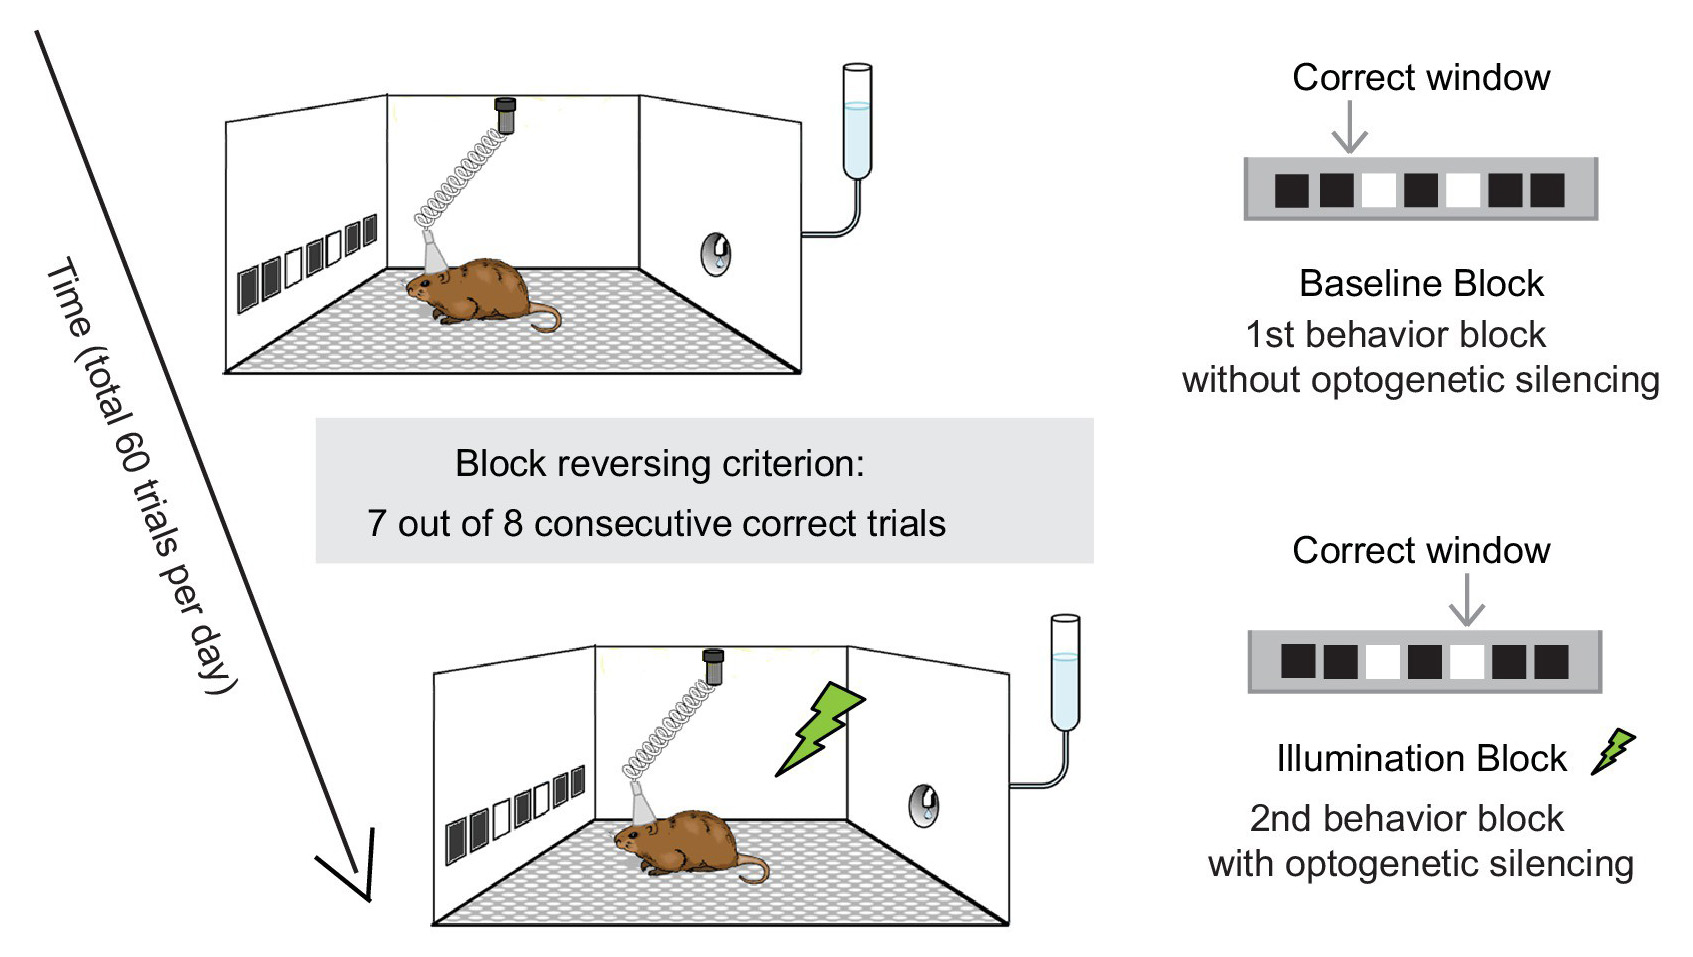
\includegraphics[width=0.5\textwidth,height=\textheight]{img/behavior-box/task-schematic.jpg}
\caption{behaviorbox schematic}
\end{figure}

\hypertarget{sec:mouse-in-a-bowl}{%
\subsection{Mouse in a Bowl}\label{sec:mouse-in-a-bowl}}

\begin{figure}
\centering

\subfloat[Raw frame of video being
tacked]{\includegraphics[width=0.3\textwidth,height=\textheight]{img/animal-tracking/01raw.jpg}}
\subfloat[Area of detected
mouse]{\includegraphics[width=0.3\textwidth,height=\textheight]{img/animal-tracking/02black-and-white.jpg}}
\subfloat[Overlay of 3 consecutive frames showing movement of mouse
between
each]{\includegraphics[width=0.3\textwidth,height=\textheight]{img/animal-tracking/03twoframes.jpg}}

\subfloat[video overlay showing tracked
points]{\includegraphics[width=0.2\textwidth,height=\textheight]{img/animal-tracking/07mousedata1close.jpg}}
\subfloat[video overlay showing tracked
points]{\includegraphics[width=0.2\textwidth,height=\textheight]{img/animal-tracking/06mousedata1.jpg}}
\subfloat[video overlay showing tracked
points]{\includegraphics[width=0.2\textwidth,height=\textheight]{img/animal-tracking/08mousedata2.jpg}}
\subfloat[video overlay showing tracked
points]{\includegraphics[width=0.2\textwidth,height=\textheight]{img/animal-tracking/09mousedata1fiberon1.jpg}}

\caption{Automated animal Tracking for ``Mouse in a bowl'' type
experiments}

\label{fig:mouse-in-a-bowl}

\end{figure}

\hypertarget{sec:spherical-treadmill}{%
\subsection{Spherical Treadmill}\label{sec:spherical-treadmill}}

\begin{figure}
\centering

\subfloat[01-treadmill-mouse-running]{\includegraphics[width=0.3\textwidth,height=\textheight]{img/spherical-treadmill-VR/01-treadmill-mouse-running.jpg}}
\subfloat[01-water-port]{\includegraphics[width=0.3\textwidth,height=\textheight]{img/spherical-treadmill-water-delivery/01-water-port.jpg}}
\subfloat[03-water-delivery-zoom]{\includegraphics[width=0.3\textwidth,height=\textheight]{img/spherical-treadmill-water-delivery/03-water-delivery-zoom.jpg}}

\caption{Spherical treadmill}

\label{fig:spherical-tradmill}

\end{figure}

\hypertarget{sec:headplate-holder}{%
\subsection{Headplate Holder}\label{sec:headplate-holder}}

\begin{figure}
\centering

\subfloat[front]{\includegraphics[width=0.3\textwidth,height=\textheight]{img/headplate-holder/photo-front.jpg}}
\subfloat[top]{\includegraphics[width=0.3\textwidth,height=\textheight]{img/headplate-holder/photo-top.jpg}}
\subfloat[bottom]{\includegraphics[width=0.3\textwidth,height=\textheight]{img/headplate-holder/photo-bottom.jpg}}

\caption{Headplate holder}

\label{fig:headplate-holder}

\end{figure}

\hypertarget{sec:motion-sensors}{%
\subsection{Motion Sensors}\label{sec:motion-sensors}}

\begin{figure}
\centering

\subfloat[01-motion-sensors-installed]{\includegraphics[width=0.3\textwidth,height=\textheight]{img/spherical-treadmill-motion-sensors/01-motion-sensors-installed.jpg}}
\subfloat[02-motion-sensors]{\includegraphics[width=0.3\textwidth,height=\textheight]{img/spherical-treadmill-motion-sensors/02-motion-sensors.jpg}}
\subfloat[Striatum\_Figure2]{\includegraphics[width=0.3\textwidth,height=\textheight]{img/spherical-treadmill-motion-sensors/Striatum_Figure2.png}}

\caption{Motion sensors}

\label{fig:motion-sensors}

\end{figure}

\hypertarget{sec:microscopes}{%
\section{Microscopes}\label{sec:microscopes}}

\hypertarget{sec:microscope-construction}{%
\subsection{Microscope Construction}\label{sec:microscope-construction}}

\begin{figure}
\centering

\subfloat[schamatic showing relation of microscope and mouse on
spherical
treadmill]{\includegraphics[width=0.5\textwidth,height=\textheight]{img/microscope/widefield_microscope_diagram.png}}

\subfloat[setup1]{\includegraphics[width=0.4\textwidth,height=\textheight]{img/microscope/setup1.jpg}}
\subfloat[setup2]{\includegraphics[width=0.4\textwidth,height=\textheight]{img/microscope/setup2.jpg}}

\subfloat[setup3-front]{\includegraphics[width=0.3\textwidth,height=\textheight]{img/microscope/setup3-front.jpg}}
\subfloat[setup3-closeup]{\includegraphics[width=0.3\textwidth,height=\textheight]{img/microscope/setup3-closeup.jpg}}
\subfloat[setup3-side]{\includegraphics[width=0.3\textwidth,height=\textheight]{img/microscope/setup3-side.jpg}}

\subfloat[setup4-front]{\includegraphics[width=0.3\textwidth,height=\textheight]{img/microscope/setup4-front.jpg}}
\subfloat[setup4-closeup]{\includegraphics[width=0.3\textwidth,height=\textheight]{img/microscope/setup4-closeup.jpg}}
\subfloat[setup4-side]{\includegraphics[width=0.3\textwidth,height=\textheight]{img/microscope/setup4-side.jpg}}

\caption{Widefield fluorescence microscope}

\label{fig:widefield-microscope}

\end{figure}

\hypertarget{sec:neural-signals-computational-considerations-interpretation-and-usage}{%
\chapter{3 Neural Signals: Computational considerations, interpretation
and
usage}\label{sec:neural-signals-computational-considerations-interpretation-and-usage}}

\hypertarget{sec:image-processing}{%
\section{Image Processing}\label{sec:image-processing}}

\hypertarget{sec:image-processing-tonemapping-and-filtering}{%
\subsection{Image Processing: Tonemapping and
Filtering}\label{sec:image-processing-tonemapping-and-filtering}}

\begin{figure}
\centering
\includegraphics[width=0.5\textwidth,height=\textheight]{img/sw-gui-interactive-parameter-selection-homomorphic-filter/Screenshot_20150608180058.png}
\caption{Screenshot\_20150608180058}
\end{figure}

\begin{figure}
\centering
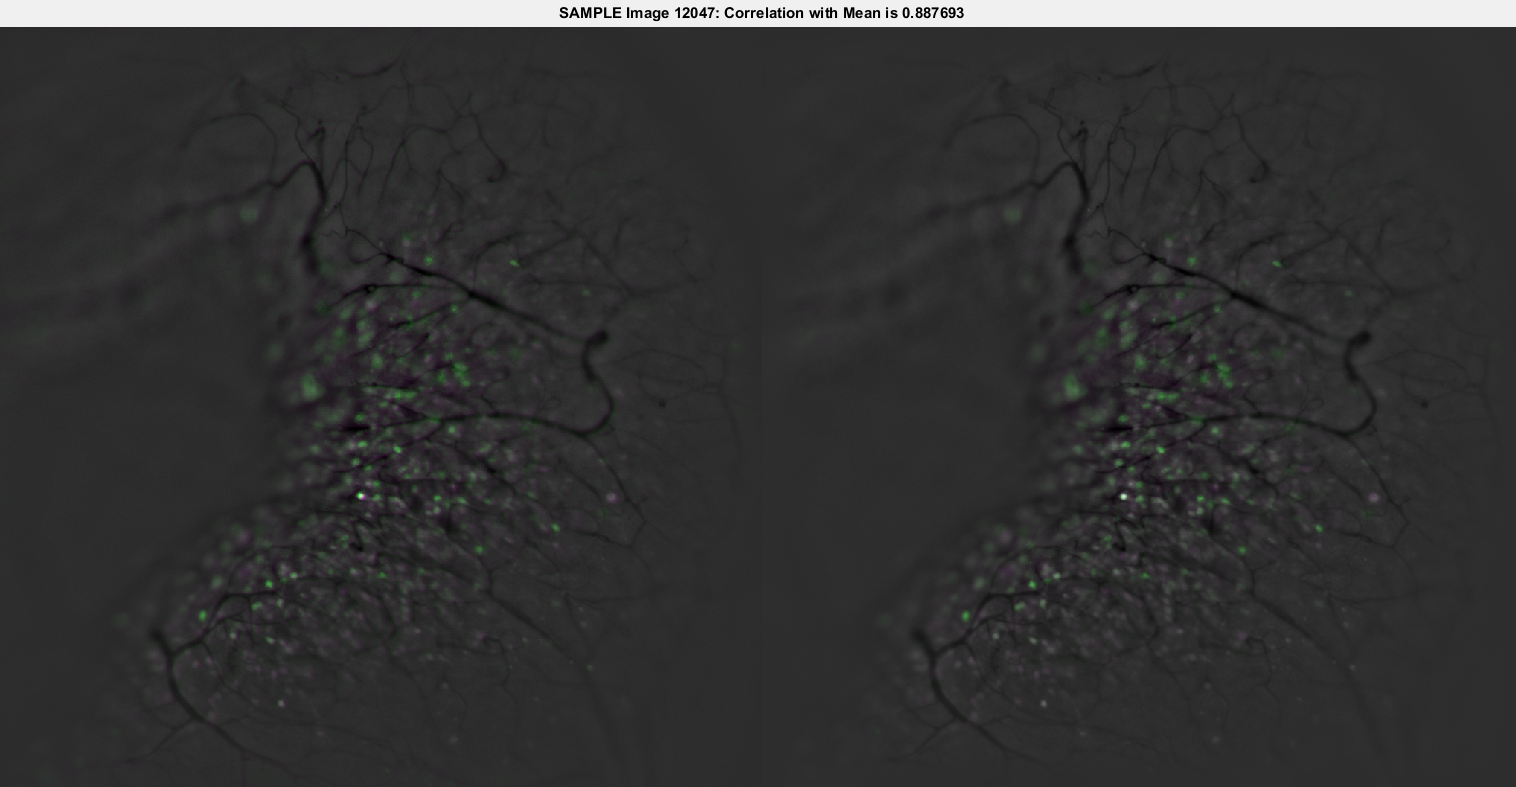
\includegraphics[width=0.5\textwidth,height=\textheight]{img/sw-fluopro/motion_correction_sample.png}
\caption{motion Correction}
\end{figure}

\begin{figure}
\centering
\includegraphics[width=0.5\textwidth,height=\textheight]{img/sw-video-processing-feature-generation.png}
\caption{feature generation}
\end{figure}

\begin{figure}
\centering
\includegraphics[width=0.5\textwidth,height=\textheight]{img/2.png}
\caption{Pixel features useful for segmentation}
\end{figure}

\begin{figure}
\centering
\includegraphics[width=0.5\textwidth,height=\textheight]{img/sw-video-processing-feature-pointwise-mutual-information.png}
\caption{sw-video-processing-feature-pointwise-mutual-information}
\end{figure}

\begin{figure}
\centering
\includegraphics[width=0.5\textwidth,height=\textheight]{img/sw-sequence-bw.png}
\caption{pixel statistics}
\end{figure}

\begin{figure}
\centering
\includegraphics[width=0.5\textwidth,height=\textheight]{img/sw-video-processing-spatially-vs-temporally-adaptive-filter.png}
\caption{sw-video-processing-spatially-vs-temporally-adaptive-filter}
\end{figure}

\begin{figure}
\centering
\includegraphics[width=0.5\textwidth,height=\textheight]{vid/trgb-013.gif}
\caption{trgb}
\end{figure}

\begin{figure}
\centering
\includegraphics[width=0.5\textwidth,height=\textheight]{img/sw-video-statistics/statistics_of_128_frames_contrast_enhanced.jpg}
\caption{central moments}
\end{figure}

\hypertarget{sec:discussion-broader-considerations-for-clinicians-engineers-and-research-scientists-preparing-to-make-use-of-an-increasingly-hyper-connected-future}{%
\chapter{4 Discussion: Broader considerations for clinicians, engineers,
and research scientists preparing to make use of an increasingly
hyper-connected
future}\label{sec:discussion-broader-considerations-for-clinicians-engineers-and-research-scientists-preparing-to-make-use-of-an-increasingly-hyper-connected-future}}

\hypertarget{sec:appendix}{%
\chapter*{Appendix}\label{sec:appendix}}
\addcontentsline{toc}{chapter}{Appendix}

\end{document}
